\documentclass[11pt]{article}
% motion_header.tex
% include this before the \begin{document} part of your LaTeX source file
%
\usepackage{fourier,ifthen,xspace,amsmath,array}
\usepackage[svgnames, dvipsnames]{xcolor}
\usepackage{graphicx}
\usepackage{siunitx}
\usepackage{xkeyval,calc,moreverb}
\usepackage[breakable,skins]{tcolorbox}
\usepackage{booktabs}
\usepackage{paralist}

% booleans we need
\newboolean{bw}
\setboolean{bw}{false}
\newboolean{solutions}

% counters

\newcounter{problemctr}

% colors

\definecolor{probLineColor}{rgb}{0.2,0.6,0.2}
\definecolor{probLabelColor}{rgb}{0,0,0} % 0.2,0.2,0.7}
\definecolor{probStatementColor}{rgb}{0,0,0}
\definecolor{solColor}{rgb}{0.2,0.6,0.2}

% lengths

\newlength{\probLineWidth} \setlength{\probLineWidth}{1.25pt}
\newlength{\solLineWidth} \setlength{\solLineWidth}{0.5pt}

% oops!
\setlength{\probLineWidth}{0pt}
\setlength{\solLineWidth}{0pt}

% commands

\newcommand{\probdir}{/Users/saeta/Documents/Courses/p24/motion/prob/}
\newcommand{\figdir}{/Users/saeta/Documents/Courses/p24/motion/figs/}
\renewcommand{\probdir}{}
\renewcommand{\figdir}{}
\newcommand{\prob}[2]{% arguments are chapter then problem
  \input{\probdir ch#1/#1P#2}
}

\newcommand{\fig}[2][2]{%
 \vspace*{-.1in}
  \begin{center}%
    \includegraphics[width=#1in]{\figdir#2}
  \end{center}%
}

\newcommand{\SolutionHead}{Solution:}
\newcommand{\theexercise}{}
\newcommand{\PNScolor}[1]{\ifthenelse{\boolean{bw}}{}{\color{#1}}}
\newcommand{\SOL}[1]{\ifthenelse{\equal{#1}{0}}%
  {
\let\solution=\comment
\let\endsolution=\endcomment
\setboolean{solutions}{false}
}%
{\setboolean{solutions}{true}%
\renewenvironment{solution}%
{\par\noindent{\color{solColor}\rule{\linewidth}{\solLineWidth}%
\ifthenelse{\equal{#1}{}}%
{}%
{\par\smallskip\noindent\textbf{\SolutionHead}}}}{}}
}


\newcommand{\val}[2]{\ensuremath{#1~\mathrm{#2}}\xspace}	% number plus unit
\newcommand{\pval}[2]{\ensuremath{\left(#1~\mathrm{#2}}\right)\xspace}
\newcommand{\hval}[2]{\ensuremath{#1$-$\mathrm{#2}}\xspace}
\newcommand{\dg}[1]{\ensuremath{#1^{\circ}}\xspace}
\newcommand{\half}{\ensuremath{\frac{1}{2}}\xspace}
\newcommand{\ux}{\ensuremath{\mathbf{\hat{x}}}\xspace}
\newcommand{\uy}{\ensuremath{\mathbf{\hat{y}}}\xspace}
\newcommand{\uz}{\ensuremath{\mathbf{\hat{z}}}\xspace}
\newcommand{\ur}{\ensuremath{\mathbf{\hat{r}}}\xspace}
\newcommand{\vv}{\ensuremath{v}\xspace}

\newcommand{\xaxis}{$x$ axis\xspace}
\newcommand{\yaxis}{$y$ axis\xspace}
\newcommand{\zaxis}{$z$ axis\xspace}
\newcommand{\xyplane}{$xy$ plane\xspace}
\newcommand{\xzplane}{$xz$ plane\xspace}
\newcommand{\DOT}{\ensuremath{\boldsymbol{\cdot}}}

\newcommand{\bo}{\ensuremath{\boldsymbol{\omega}}\xspace}
\newcommand{\bO}{\ensuremath{\boldsymbol{\Omega}}\xspace}
\newcommand{\VEC}[1]{\ensuremath{\mathbf{#1}}\xspace}
\newcommand{\AU}{\ensuremath{\mathrm{A.U.}}\xspace}
\newcommand{\DB}{\ensuremath{\mathrm{dB}}\xspace}
\newcommand{\degC}[1]{\ensuremath{#1^{\circ}\mathrm{C}}\xspace}


% environments
\newcommand{\problabel}{Problem}
\newenvironment{problem}[1][]%
{
  \begingroup\refstepcounter{problemctr}
  \ifthenelse{\boolean{solutions}}%
    {
      {\vspace*{-10pt}\noindent\PNScolor{probLineColor}%
        \rule[-5pt]{\linewidth}{\probLineWidth}}
    }{}
  \begin{list}{%
      \PNScolor{probLabelColor}\textbf{\problabel\theexercise}%
    }{%
      \setlength{\labelsep}{0pt}%
      \setlength{\leftmargin}{0in}%
      \setlength{\labelwidth}{0pt}%
      \setlength{\listparindent}{0pt}
    }%
    \PNScolor{probStatementColor}%
	\item%
	\ifthenelse{\equal{#1}{}}%
      {}%
      {\textbf{ -- #1}}%
      \quad
}%
{%
  \end{list}\endgroup%
  \PNScolor{black}%
}

\newcommand{\PAGE}[2]{#1-#2\xspace}

\newenvironment{solution}{}{}
\newenvironment{question}{\renewcommand{\problabel}{Question}\begin{problem}}
{\end{problem}\renewcommand{\problabel}{Problem}}

\SOL{1} % show solution

\makeatletter
\newlength\rpLW
\newlength\rpRW
\newlength\rpgap
\newcommand{\rprcent}{0}
\newcommand{\rplcent}{0}
\define@key{rp}{lwidth}{\setlength{\rpLW}{#1}  \setlength{\rpRW}{\columnwidth-#1-\rpgap}}
\define@key{rp}{rwidth}{\setlength{\rpRW}{#1} \setlength{\rpLW}{\columnwidth-#1-\rpgap}}
 \define@key{rp}{lvert}{\def\LeftVerticalCode{#1}}
\define@key{rp}{rvert}{\def\RightVerticalCode{#1}}
\define@key{rp}{gap}{\setlength{\rpgap}{#1}}
\define@key{rp}{rcent}{\def\rprcent{#1}}
\define@key{rp}{lcent}{\def\rplcent{#1}}
\setkeys{rp}{rwidth=2in, lvert=c, rvert=t, gap=0.25in, rcent=0, lcent=0}
\makeatother

\newcommand\rp[3][]{%
  \setkeys{rp}{#1}
  \noindent \parbox[\LeftVerticalCode]{\rpLW}%
  {\ifthenelse{\equal{\rplcent}{0}}%
  {#2}%
  { \begin{center}#2\end{center} }%
  }%
  \hspace*{\rpgap}%
  \parbox[\RightVerticalCode]{\rpRW}%
  {\ifthenelse{\equal{0}{\rprcent}}%
  {#3}%
  {\begin{center} #3 \end{center}}}%
}

\newcommand{\DD}{\ensuremath{d}}		% differential d without leading space
\newcommand{\dd}{\ensuremath{\,\DD}}	% differential d

\newcommand{\deriv}[3][]{\ensuremath{%
	\ifthenelse{\equal{#1}{}}{\frac{\DD #2}{\DD #3}}
	{\frac{\DD^{#1} #2}{\DD #3^{#1}}}}}

\newcommand{\pd}[3][]{\ensuremath{%
	\ifthenelse{\equal{#1}{}}{\frac{\partial #2}{\partial #3}}
	{\partial #2 / \partial #3}}}

\newcommand{\so}{\ensuremath{\qquad\Longrightarrow\qquad}}
\newcommand{\uth}{\ensuremath{\boldsymbol{\hat{\theta}}}\xspace}
\newcommand{\eref}[2][]{%
	\ifthenelse{\equal{#1}{}}%
	{Eq.~(\ref{eq:#2})}%
	{Equation~(\ref{eq:#2})}\xspace}
\newcommand{\cross}{\ensuremath{\times}\xspace}
\newcommand{\into}{\ensuremath{\hat{\otimes}}}	% direction symbols
\newcommand{\outof}{\ensuremath{\hat{\odot}}}
\newcommand{\ds}{\displaystyle}

\newcommand{\xdd}{\ensuremath{\ddot{x}}\xspace}
\newcommand{\thdd}{\ensuremath{\ddot{\theta}}\xspace} % Download this file from physics.hmc.edu/motion/ page
\usepackage{tikz}

\usetikzlibrary{arrows,calc}
                	\tikzset{%
                         every picture/.style={>=stealth'},
                                        vel/.style={->,line width=2pt,color=DarkBlue},
                  force/.style={line width=1.5pt,color=blue,->},
                  coord/.style={color=green!40!black,|->},
                  accel/.style={->,line width=3pt,color=gray},
                  photon/.style={line width=1.5pt,color=DarkRed,decorate,decoration={snake,post length=0.1in}},
                  spring/.style={decorate,decoration={coil,aspect=0.3,segment length=2mm,amplitude=2mm}},
                  traj/.style={dashed, color=gray, line width=1pt}
                }
                
\usepackage{fullpage}
\setlength{\parskip}{6pt}
\setlength{\parindent}{0pt}
\usepackage[margin=1in]{geometry}
\usepackage{graphicx}
\usepackage{enumerate}
\usepackage{marvosym}
\usepackage{amssymb}
\usepackage{wasysym}
\usepackage{gensymb}
\usepackage{mathrsfs}
\usepackage{scrextend}
\usepackage{mathtools}
\usepackage{pgfplots}
\usepackage{xspace}
\usepackage[colorlinks]{hyperref}

% --- style --- %
\renewcommand{\labelenumi}{{ (\alph{enumi})}}
\newcommand{\sand}{\quad \mbox{ and } \quad}
\newcommand{\be}{\begin{enumerate}[a) ]}
\newcommand{\ee}{\end{enumerate}}
\def\bal#1\eal{\begin{align*}#1\end{align*}}
\allowdisplaybreaks

% --- making \xi look less awful --- %
\DeclareSymbolFont{CMletters}{OML}{cmm}{m}{it}
\DeclareMathSymbol{\xi}{\mathord}{CMletters}{"18}

% --- math --- %
\newcommand{\Z}{\mathbb{Z}}
\newcommand{\R}{\mathbb{R}}
\newcommand{\C}{\mathbb{C}}
\newcommand{\Q}{\mathbb{Q}}


\newcommand{\Lt}[1]{\mathcal{L}\crb{#1}}
\newcommand{\ilt}[1]{\mathcal{L}^{-1}\crb{#1}}

\newcommand{\pn}[1]{\left( #1 \right)}
\newcommand{\sqb}[1]{\left[ #1 \right]}
\newcommand{\crb}[1]{\left\{ #1 \right\}}
\newcommand{\lra}[1]{\left\langle #1 \right\rangle}
\newcommand{\magn}[1]{\left\lVert #1 \right\rVert}

\def\multiset#1#2{\ensuremath{\left(\kern-.3em\left(\genfrac{}{}{0pt}{}{#1}{#2}\right)\kern-.3em\right)}}

\newcommand{\pdr}[2]{\frac{\partial #1}{\partial #2}}
\newcommand{\im}[1]{\text{im}\pn{#1}}
\newcommand{\m}[1]{\Z/#1\Z}


\DeclareMathOperator{\proj}{proj}
\newcommand{\vectorproj}[2][]{\proj_{\VEC{#1}}\VEC{#2}}

\newenvironment{amatrix}[1]{%
  \left(\begin{array}{@{}*{#1}{c}|c@{}}
}{%
  \end{array}\right)
}

\makeatletter
\renewcommand*\env@matrix[1][*\c@MaxMatrixCols c]{%
  \hskip -\arraycolsep
  \let\@ifnextchar\new@ifnextchar
  \array{#1}}
\makeatother

\newcommand{\spn}[1]{\text{span}\pn{#1}}

\newcommand*\Heq{\ensuremath{\overset{\kern2pt H}{=}}}

\newcommand{\distil}{\sqrt{1-v^2/c^2}}
\newcommand{\distilf}[1]{\sqrt{1-(#1)^2}}
\newcommand{\lorentz}{\frac{1}{\distil}}
\newcommand{\lorentzf}[1]{\frac{1}{\sqrt{1-(#1)^2}}}


\begin{document}

\noindent{\large Problem Set 8, 29 October 2018\hfill Name: \underline{\hspace{3cm}} ,  Section: \underline{\hspace{5mm}} }
\vspace*{0.25in}


\begin{problem}[(E34.30)]
A long solenoid has a diameter of 12.6 cm. When a current $i$ is passed through its windings, a
uniform magnetic field $B = \val{28.6}{mT}$ is produced in its interior. By decreasing $i$, the field is caused
to decrease at the rate $\val{6.51}{mT/s}$. Calculate the magnitude of the induced electric field
\be
\item 2.20 cm and
\item 8.20 cm from the axis of the solenoid.
\ee
\end{problem}


% Your solution starts here %%%%%%%%%%%%%%%%%%%%%%%%%%%%%%%%%%%%%%%%%%%%%%%%%%
\textbf{Solution:}\\

\clearpage
% Your solution ends here %%%%%%%%%%%%%%%%%%%%%%%%%%%%%%%%%%%%%%%%%%%%%%%%%%

\begin{problem}[(P34.6)*]
The figure below shows two parallel loops of wire having a common axis. The smaller loop (radius $r$)
is above the larger loop (radius $R$), by a difference $x \gg R$. Consequently the magnetic field, due
to the current $i$ in the larger loop, is nearly constant throughout the smaller loop and equal to the
value on the axis. Suppose that $x$ is increasing at the constant rate $dx/dt = v$.
\be
\item Determine the magnetic flux across the area bounded by the smaller loop as a function of $x$.
\item Compute the emf generated in the smaller loop.
\item Determine the direction of the induced current flowing in the smaller loop.
\ee
\begin{center}
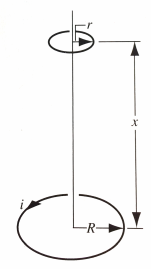
\includegraphics[scale=0.5]{prob2.png}
\end{center}
\end{problem}


% Your solution starts here %%%%%%%%%%%%%%%%%%%%%%%%%%%%%%%%%%%%%%%%%%%%%%%%%%
\textbf{Solution:}\\

\clearpage
% Your solution ends here %%%%%%%%%%%%%%%%%%%%%%%%%%%%%%%%%%%%%%%%%%%%%%%%%%

\begin{problem}[(P34.9)]
\be
\item Find an expression for the energy density as a function of the radial distance $r$ for a toroid
of rectangular cross section.
\item Integrating the energy density over the volume of the toroid, calculate the total energy stored
in the field of the toroid.
\item Using Eq. 36-10, evaluate the energy stored in the toroid directly from the inductance and
compare with (b).
\ee
\end{problem}


% Your solution starts here %%%%%%%%%%%%%%%%%%%%%%%%%%%%%%%%%%%%%%%%%%%%%%%%%%
\textbf{Solution:}\\

\clearpage
% Your solution ends here %%%%%%%%%%%%%%%%%%%%%%%%%%%%%%%%%%%%%%%%%%%%%%%%%%

\begin{problem}[(E36.21)]
In the circuit shown in the figure below, $\mathcal{E} = \val{10}{V}$, $R_1 = 5.0\Omega$, $R_2 = 10 \Omega$ , and $L = \val{5.0}{H}$. For the two
separate conditions
\be
\item[(I) ] switch S just closed and
\item[(II) ] switch S closed for a long time,
\ee
calculate
\be
\item the current $i_1$ through $R_1$,
\item the current $i_2$ through $R_2$,
\item the current $i$ through the switch,
\item the potential difference across $R_2$,
\item the potential difference across $L$, and
\item $di_2/dt$.
\ee
\begin{center}
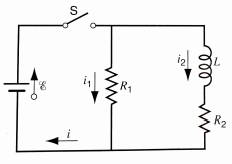
\includegraphics[scale=0.6]{prob4.png}
\end{center}
\end{problem}


% Your solution starts here %%%%%%%%%%%%%%%%%%%%%%%%%%%%%%%%%%%%%%%%%%%%%%%%%%
\textbf{Solution:}\\

\clearpage
% Your solution ends here %%%%%%%%%%%%%%%%%%%%%%%%%%%%%%%%%%%%%%%%%%%%%%%%%%

\begin{problem}[\P(P38.3)]
The capacitor in the figure below consisting of two circular plates with radius $R = \val{18.2}{cm}$ is connected
to a source of emf  $\mathcal{E} = \mathcal{E}_m \sin(\omega t)$, where $\mathcal{E}_m = \val{225}{V}$ and $\omega = \val{128}{rad/s}$. The maximum value of
the displacement current is $i_d = \val{7.63}{\mu A}$. Neglect fringing of the electric field at the edges of the
plates.
\be
\item What is the maximum value of the current $i$?
\item What is the maximum value of $d\Phi_E/dt$, where $\Phi_E$ is the electric flux through the region
between the plates?
\item What is the separation $d$ between the plates?
\item Find the maximum value of the magnitude of \textbf{B} between the plates at a distance $r = \val{11.0}{cm}$
from the center.
\ee
\begin{center}
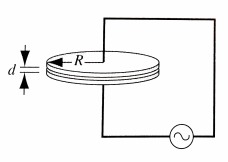
\includegraphics[scale=0.6]{prob5.png}
\end{center}
\end{problem}


% Your solution starts here %%%%%%%%%%%%%%%%%%%%%%%%%%%%%%%%%%%%%%%%%%%%%%%%%%
\textbf{Solution:}\\

\clearpage
% Your solution ends here %%%%%%%%%%%%%%%%%%%%%%%%%%%%%%%%%%%%%%%%%%%%%%%%%%

\begin{problem}[\P Supplementary Problem 3]
A parallel plate capacitor has circular plates of radius $R$ and separation $d$. The capacitor is
connected to a battery of voltage $V$ and then disconnected so that the charge ought to remain
constant. The air is humid, however, and therefore slightly conducting; thus the stored charge
leaks back across the air gap between the capacitor plates at rate $i_{\text{leak}}$. Assume that this leakage
current is uniformly distributed across the area of the plates. Find the magnetic field everywhere
between the plates.
\end{problem}


% Your solution starts here %%%%%%%%%%%%%%%%%%%%%%%%%%%%%%%%%%%%%%%%%%%%%%%%%%
\textbf{Solution:}\\

\clearpage
% Your solution ends here %%%%%%%%%%%%%%%%%%%%%%%%%%%%%%%%%%%%%%%%%%%%%%%%%%


\end{document}